%\documentclass[handout]{beamer}
%\documentclass[handout,10pt,slidestop,mathserif]{beamer}
%\usepackage{pgfpages}
%\pgfpagesuselayout{2 on 1}
\documentclass[10pt,slidestop,mathserif,c]{beamer}
\usetheme{Madrid}
\usecolortheme{seahorse}

\usepackage{tabularx}
\usepackage{verbatim}
\usepackage{graphics}
\usepackage{graphicx}
\usepackage{Sweave}
\usepackage{moreverb}
\usepackage{pgf}
\usepackage{tikz}
\usepackage{Sweave}
%\SweaveOpts{prefix.string=figures/}

\newcommand{\putat}[3]{\begin{picture}(0,0)(0,0)\put(#1,#2){#3}\end{picture}}
  
\newenvironment{changemargin}[2]{%
  \begin{list}{}{%
    \setlength{\topsep}{0pt}%
    \setlength{\leftmargin}{#1}%
    \setlength{\rightmargin}{#2}%
    \setlength{\listparindent}{\parindent}%
    \setlength{\itemindent}{\parindent}%
    \setlength{\parsep}{\parskip}%
  }%
  \item[]}{\end{list}}

%% Define a new 'leo' style for the package that will use a smaller font.
\makeatletter
\def\url@leostyle{%
  \@ifundefined{selectfont}{\def\UrlFont{\sf}}{\def\UrlFont{\tiny\ttfamily}}}
\makeatother

\title{EPSY 887: Computation Statistics}
\subtitle{Reshaping \& Merging Data}
\author[Jason Bryer]{Jason Bryer}
\institute[Jason.Bryer.org]{\url{http://github.com/jbryer/CompStats}\\\href{mailto:jason@bryer.org}{jason@bryer.org}}
\date[Feb 11, 2013]{Week 3\\February 11, 2013}

\begin{document}

\AtBeginSection[]
{
   \begin{frame}
       \frametitle{Outline}
       \tableofcontents[currentsection,currentsubsections]
   \end{frame}
}


\frame{\titlepage}
\frame{\frametitle{Agenda}\tableofcontents[hideallsubsections]}

\section{Sorting Data}

\begin{frame}[fragile,containsverbatim]
	\frametitle{Sorting Data}
	The \texttt{order} function will return a vector with the position of the elements ordered.
\begin{Schunk}
\begin{Sinput}
> test <- c("s","t","a","t","i","s","t","i","c","s")
> test
\end{Sinput}
\begin{Soutput}
 [1] "s" "t" "a" "t" "i" "s" "t" "i" "c" "s"
\end{Soutput}
\begin{Sinput}
> order(test)
\end{Sinput}
\begin{Soutput}
 [1]  3  9  5  8  1  6 10  2  4  7
\end{Soutput}
\begin{Sinput}
> test[order(test)]
\end{Sinput}
\begin{Soutput}
 [1] "a" "c" "i" "i" "s" "s" "s" "t" "t" "t"
\end{Soutput}
\end{Schunk}
\end{frame}

\begin{frame}[fragile,containsverbatim]
	\frametitle{Sorting a Data Frame}
	Using the \texttt{mtcars} dataset, first we'll sort by mpg

\begin{Schunk}
\begin{Sinput}
> mtcars.mpg <- mtcars[order(mtcars$mpg),]
> head(mtcars.mpg)
\end{Sinput}
\begin{Soutput}
                    mpg cyl disp  hp drat  wt qsec vs am gear carb
Cadillac Fleetwood   10   8  472 205  2.9 5.2   18  0  0    3    4
Lincoln Continental  10   8  460 215  3.0 5.4   18  0  0    3    4
Camaro Z28           13   8  350 245  3.7 3.8   15  0  0    3    4
Duster 360           14   8  360 245  3.2 3.6   16  0  0    3    4
Chrysler Imperial    15   8  440 230  3.2 5.3   17  0  0    3    4
Maserati Bora        15   8  301 335  3.5 3.6   15  0  1    5    8
\end{Soutput}
\end{Schunk}
\end{frame}


\begin{frame}[fragile,containsverbatim]
	\frametitle{Sorting a Data Frame}

	By default the \texttt{order} function returns a list in ascending order. To return in descending order specify the \texttt{decreasing=TRUE} parameter.

\begin{Schunk}
\begin{Sinput}
> mtcars.mpg.desc <- mtcars[order(mtcars$mpg, decreasing=TRUE),]
> head(mtcars.mpg.desc)
\end{Sinput}
\begin{Soutput}
               mpg cyl disp  hp drat  wt qsec vs am gear carb
Toyota Corolla  34   4   71  65  4.2 1.8   20  1  1    4    1
Fiat 128        32   4   79  66  4.1 2.2   19  1  1    4    1
Honda Civic     30   4   76  52  4.9 1.6   19  1  1    4    2
Lotus Europa    30   4   95 113  3.8 1.5   17  1  1    5    2
Fiat X1-9       27   4   79  66  4.1 1.9   19  1  1    4    1
Porsche 914-2   26   4  120  91  4.4 2.1   17  0  1    5    2
\end{Soutput}
\end{Schunk}

\end{frame}



\section{Merging data}

\begin{frame}
	\frametitle{Merging Data}
	
	The \texttt{merge} function will combine two data frames by one or more common key variables. For example, consider two data frames, one listing authors and another listing books. We may wish to combine these two data frames into a single data frame. We can link them by the author's name.
\end{frame}


\begin{frame}[fragile,containsverbatim]
	\frametitle{Merging Data}

\begin{Schunk}
\begin{Sinput}
> authors
\end{Sinput}
\begin{Soutput}
   surname nationality deceased
1    Tukey          US      yes
2 Venables   Australia       no
3  Tierney          US       no
4   Ripley          UK       no
5   McNeil   Australia       no
\end{Soutput}
\begin{Sinput}
> books
\end{Sinput}
\begin{Soutput}
      name                         title     other.author
1    Tukey     Exploratory Data Analysis             <NA>
2 Venables Modern Applied Statistics ...           Ripley
3  Tierney                     LISP-STAT             <NA>
4   Ripley            Spatial Statistics             <NA>
5   Ripley         Stochastic Simulation             <NA>
6   McNeil     Interactive Data Analysis             <NA>
7   R Core          An Introduction to R Venables & Smith
\end{Soutput}
\end{Schunk}
\end{frame}

\begin{frame}[fragile,containsverbatim]
	\frametitle{Merging Data}

\begin{Schunk}
\begin{Sinput}
> merge(authors, books, by.x = "surname", by.y = "name")
\end{Sinput}
\begin{Soutput}
   surname nationality deceased                         title
1   McNeil   Australia       no     Interactive Data Analysis
2   Ripley          UK       no            Spatial Statistics
3   Ripley          UK       no         Stochastic Simulation
4  Tierney          US       no                     LISP-STAT
5    Tukey          US      yes     Exploratory Data Analysis
6 Venables   Australia       no Modern Applied Statistics ...
  other.author
1         <NA>
2         <NA>
3         <NA>
4         <NA>
5         <NA>
6       Ripley
\end{Soutput}
\end{Schunk}
\end{frame}

\begin{frame}[fragile,containsverbatim]
	\frametitle{Merging Data}

\begin{Schunk}
\begin{Sinput}
> merge(books, authors, by.x = "name", by.y = "surname")
\end{Sinput}
\begin{Soutput}
      name                         title other.author nationality
1   McNeil     Interactive Data Analysis         <NA>   Australia
2   Ripley            Spatial Statistics         <NA>          UK
3   Ripley         Stochastic Simulation         <NA>          UK
4  Tierney                     LISP-STAT         <NA>          US
5    Tukey     Exploratory Data Analysis         <NA>          US
6 Venables Modern Applied Statistics ...       Ripley   Australia
  deceased
1       no
2       no
3       no
4       no
5      yes
6       no
\end{Soutput}
\end{Schunk}
\end{frame}

\begin{frame}[fragile,containsverbatim]
	\frametitle{Merging Data}

\begin{Schunk}
\begin{Sinput}
> merge(authors, books, by.x = "surname", by.y = "name", all=TRUE)
\end{Sinput}
\begin{Soutput}
   surname nationality deceased                         title
1   McNeil   Australia       no     Interactive Data Analysis
2   R Core        <NA>     <NA>          An Introduction to R
3   Ripley          UK       no            Spatial Statistics
4   Ripley          UK       no         Stochastic Simulation
5  Tierney          US       no                     LISP-STAT
6    Tukey          US      yes     Exploratory Data Analysis
7 Venables   Australia       no Modern Applied Statistics ...
      other.author
1             <NA>
2 Venables & Smith
3             <NA>
4             <NA>
5             <NA>
6             <NA>
7           Ripley
\end{Soutput}
\end{Schunk}
\end{frame}

\section{Reshaping Data}

\begin{frame}[fragile,containsverbatim]
	\frametitle{Transpose}
	The \texttt{t} function will transpose a matrix or data frame. That is, rows become columns and columns become rows.
	
\begin{Schunk}
\begin{Sinput}
> head(mtcars)
\end{Sinput}
\begin{Soutput}
                  mpg cyl disp  hp drat  wt qsec vs am gear carb
Mazda RX4          21   6  160 110  3.9 2.6   16  0  1    4    4
Mazda RX4 Wag      21   6  160 110  3.9 2.9   17  0  1    4    4
Datsun 710         23   4  108  93  3.9 2.3   19  1  1    4    1
Hornet 4 Drive     21   6  258 110  3.1 3.2   19  1  0    3    1
Hornet Sportabout  19   8  360 175  3.1 3.4   17  0  0    3    2
Valiant            18   6  225 105  2.8 3.5   20  1  0    3    1
\end{Soutput}
\begin{Sinput}
> head(t(mtcars))
\end{Sinput}
\begin{Soutput}
     Mazda RX4 Mazda RX4 Wag Datsun 710 Hornet 4 Drive
mpg       21.0          21.0       22.8           21.4
cyl        6.0           6.0        4.0            6.0
disp     160.0         160.0      108.0          258.0
hp       110.0         110.0       93.0          110.0
drat       3.9           3.9        3.9            3.1
wt         2.6           2.9        2.3            3.2
     Hornet Sportabout Valiant Duster 360 Merc 240D Merc 230 Merc 280
mpg               18.7    18.1       14.3      24.4     22.8     19.2
cyl                8.0     6.0        8.0       4.0      4.0      6.0
disp             360.0   225.0      360.0     146.7    140.8    167.6
hp               175.0   105.0      245.0      62.0     95.0    123.0
drat               3.1     2.8        3.2       3.7      3.9      3.9
wt                 3.4     3.5        3.6       3.2      3.1      3.4
     Merc 280C Merc 450SE Merc 450SL Merc 450SLC Cadillac Fleetwood
mpg       17.8       16.4       17.3        15.2               10.4
cyl        6.0        8.0        8.0         8.0                8.0
disp     167.6      275.8      275.8       275.8              472.0
hp       123.0      180.0      180.0       180.0              205.0
drat       3.9        3.1        3.1         3.1                2.9
wt         3.4        4.1        3.7         3.8                5.2
     Lincoln Continental Chrysler Imperial Fiat 128 Honda Civic
mpg                 10.4              14.7     32.4        30.4
cyl                  8.0               8.0      4.0         4.0
disp               460.0             440.0     78.7        75.7
hp                 215.0             230.0     66.0        52.0
drat                 3.0               3.2      4.1         4.9
wt                   5.4               5.3      2.2         1.6
     Toyota Corolla Toyota Corona Dodge Challenger AMC Javelin
mpg            33.9          21.5             15.5        15.2
cyl             4.0           4.0              8.0         8.0
disp           71.1         120.1            318.0       304.0
hp             65.0          97.0            150.0       150.0
drat            4.2           3.7              2.8         3.1
wt              1.8           2.5              3.5         3.4
     Camaro Z28 Pontiac Firebird Fiat X1-9 Porsche 914-2 Lotus Europa
mpg        13.3             19.2      27.3          26.0         30.4
cyl         8.0              8.0       4.0           4.0          4.0
disp      350.0            400.0      79.0         120.3         95.1
hp        245.0            175.0      66.0          91.0        113.0
drat        3.7              3.1       4.1           4.4          3.8
wt          3.8              3.8       1.9           2.1          1.5
     Ford Pantera L Ferrari Dino Maserati Bora Volvo 142E
mpg            15.8         19.7          15.0       21.4
cyl             8.0          6.0           8.0        4.0
disp          351.0        145.0         301.0      121.0
hp            264.0        175.0         335.0      109.0
drat            4.2          3.6           3.5        4.1
wt              3.2          2.8           3.6        2.8
\end{Soutput}
\end{Schunk}

\end{frame}

\begin{frame}[fragile,containsverbatim]
	\frametitle{Reshape}
	The \texttt{reshape} and \texttt{reshape2} packages provide a robust set of functions to melt and cast data frames.
	
\begin{Schunk}
\begin{Sinput}
> mydata <- data.frame(id=c(1,1,2,2), time=c(1,2,1,2), x1=c(5,3,6,2), x2=c(6,5,1,4))
> mydata
\end{Sinput}
\begin{Soutput}
  id time x1 x2
1  1    1  5  6
2  1    2  3  5
3  2    1  6  1
4  2    2  2  4
\end{Soutput}
\begin{Sinput}
> require(reshape2)
\end{Sinput}
\end{Schunk}

\end{frame}


\begin{frame}[fragile,containsverbatim]
	\frametitle{Melting}
	
\begin{Schunk}
\begin{Sinput}
> mydata.melted <- melt(mydata, id=c("id","time"))
> mydata.melted
\end{Sinput}
\begin{Soutput}
  id time variable value
1  1    1       x1     5
2  1    2       x1     3
3  2    1       x1     6
4  2    2       x1     2
5  1    1       x2     6
6  1    2       x2     5
7  2    1       x2     1
8  2    2       x2     4
\end{Soutput}
\end{Schunk}

\end{frame}

\begin{frame}[fragile,containsverbatim]
	\frametitle{Casting}
	The \texttt{reshape2} package has two functions for casting depending on the desired output. The\texttt{dcast} function will return a data frame and the \texttt{acast} function will return an array or matrix.

\begin{Schunk}
\begin{Sinput}
> dcast(mydata.melted, id ~ variable, mean)
\end{Sinput}
\begin{Soutput}
  id x1  x2
1  1  4 5.5
2  2  4 2.5
\end{Soutput}
\begin{Sinput}
> dcast(mydata.melted, time ~ variable, mean)
\end{Sinput}
\begin{Soutput}
  time  x1  x2
1    1 5.5 3.5
2    2 2.5 4.5
\end{Soutput}
\end{Schunk}

\end{frame}


\section{ggplot2: A Grammar of Graphics}

\begin{frame}[containsverbatim,fragile]
	\frametitle{ggplot2: A Grammar of Graphics}
	\begin{itemize}
		\item ggplot2 is an R package that provides an alternative framework based upon Wilkinson's (2005) Grammar of Graphics.
		\item ggplot2 is, in general, more flexible for creating "prettier" and complex plots.
		\item Works by creating layers of different types of objects/geometries (i.e. bars, points, lines, polygons, etc.)
		\item ggplot2 has at least three ways of creating plots:
			\begin{enumerate}
				\item \begin{verbatim} qplot \end{verbatim} 
				\item \begin{verbatim} ggplot(...) + geom_XXX(...) + ... \end{verbatim}
				\item \begin{verbatim} ggplot(...) + layer(...) \end{verbatim}
			\end{enumerate}
		We will focus only on the second.
	\end{itemize}
\end{frame}

\begin{frame}[containsverbatim,fragile]
	\frametitle{First Example}
\begin{figure}
\begin{Schunk}
\begin{Sinput}
> data(diamonds)
> p <- ggplot(diamonds, aes(x=carat,y=price,colour=cut)) + 
   	geom_point()
> print(p)
\end{Sinput}
\end{Schunk}
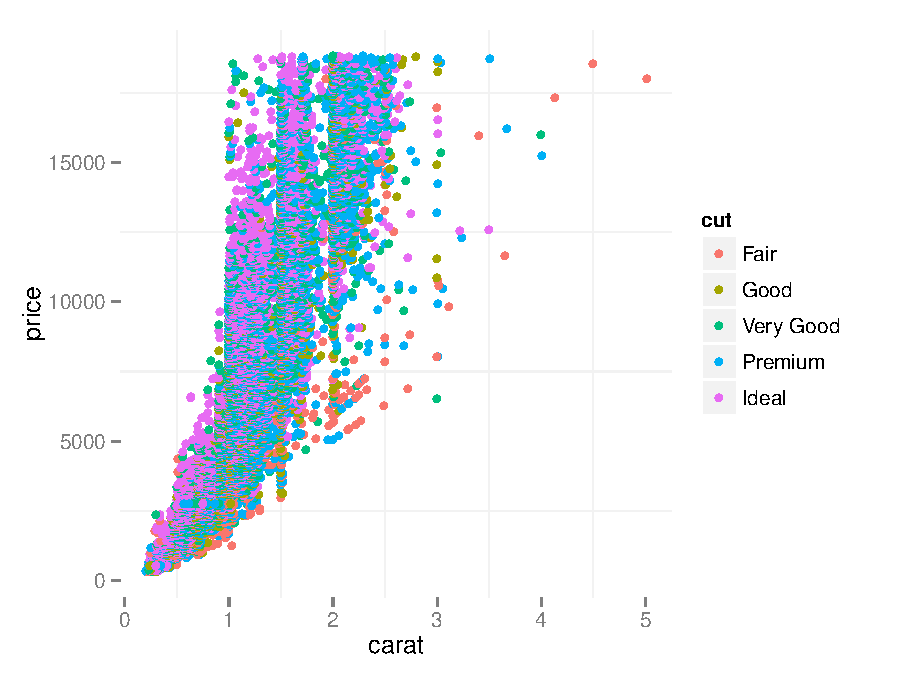
\includegraphics{Slides-ggplot-fig1}
\end{figure}
\end{frame}

\begin{frame}[containsverbatim,fragile]
	\frametitle{First Example}
\begin{figure}
\begin{Schunk}
\begin{Sinput}
> p <- p + facet_wrap(~cut) + 
   	ggtitle("First example")
> print(p)
\end{Sinput}
\end{Schunk}
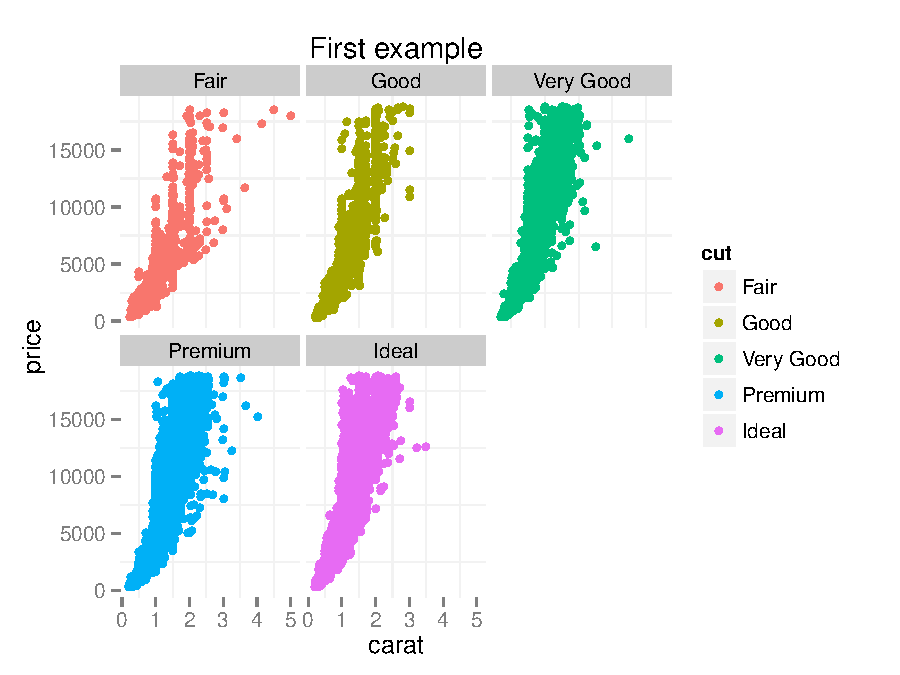
\includegraphics{Slides-ggplot-fig2}
\end{figure}
\end{frame}

\begin{frame}[containsverbatim,fragile]
	\frametitle{Parts of a ggplot2 statement}
	\begin{itemize}
		\item<+-| alert@+> Data \begin{verbatim} ggplot(myDataFrame, aes(x=x, y=y) \end{verbatim}
		\item<+-| alert@+> Layers \begin{verbatim} geom_point(), geom_histogram() \end{verbatim}
		\item<+-| alert@+> Facets \begin{verbatim} facet_wrap(~ cut), facet_grid(~ cut) \end{verbatim}
		\item<+-| alert@+> Scales \begin{verbatim} scale_y_log10() \end{verbatim}
		\item<+-| alert@+> Other options \begin{verbatim} ggtitle("my title"), ylim(c(0, 10000)), xlab("x-axis label") \end{verbatim}
	\end{itemize}
\end{frame}

\begin{frame}[containsverbatim,fragile]
	\frametitle{Lots of geoms}
	\begin{columns}[c]
	\column{1.5in}
\begin{verbatim} 
geom_abline
geom_jitter
geom_area
geom_line
geom_bar	
geom_linerange
geom_bin2d
geom_path 
geom_blank
geom_point 
geom_boxplot
geom_pointrange 
geom_contour
geom_polygon 
geom_crossbar
geom_quantile 
\end{verbatim}
\column{1.5in}
\begin{verbatim}
geom_density
geom_rect 
geom_density2d
geom_ribbon
geom_errorbar
geom_rug
geom_errorbarh
geom_segment 
geom_freqpoly
geom_smooth 
geom_hex
geom_step
geom_histogram
geom_text 
geom_hline
geom_tile
geom_vline
\end{verbatim}
\end{columns}
\end{frame}




%\begin{frame}[c]
%	\LARGE{Thank You}\\
%	\normalsize
%	Jason Bryer (jason@bryer.org)\\
%	\url{http://jbryer.github.com}
%\end{frame}

\end{document}
